%!TEX root = ../authorinstr.tex

\section{Continuous Actor Critic Learning Automaton}
A well established algorithm in Reinforcement Learning (RL) is Continuous Actor Critic Learning Automaton (CACLA)~\cite{van2007reinforcement}. CACLA deals with undiscretized continuous state and action spaces. It implements an Actor Critic (AC) system in which both the Actor and Critic are represented by a Multi-Layer Perceptron. In an AC system, the Actor is responsible for selecting the current action given the policy and the Critic is used in the calculation of the Temporal Difference (TD)-error which drives the learning of the Actor. The TD-learning rule is characterized by equation \eqref{eq:td}, where $\delta_{t}$ is the TD-difference error as written in \eqref{eq:tderror}. The Actor-Critic system allows for a seperation between the representation of the policy and the value function. A visualization of the Actor-Critic system is shown in Figure~\ref{fig:actorcriticsystem}. In RL problems it is important to be aware of the exploration versus exploitation trade-off; meaning that a decision has to be made between exploration which might lead to an improvement of the current policy or simply the action is selected according to the current policy. An exploration technique that is used often in CACLA is Gaussian Exploration, meaning that an action is calculated around the best action that the current policy provides. To pick a value around the best action, a sample is chosen from a gaussian distribution $N(action, \sigma)$, where $\sigma$ denotes the standard deviation of the distribution. The sign of the TD-error ($\delta_{t} > 0$) is used to determine whether the policy of the Actor has to be updated. To update the Actor in a connectionist way, the performed action $a_{t}$ is used as the target when backpropgating the error using the state $s_{t}$ as input. Since CACLA is an online RL algorithm, the data that is gathered from the interaction of the agent with the environment is used immediately to update the Critic and possibly the Actor. 

\begin{equation}
\label{eq:td}
V(s_{t+1}) = V(s_t) + \alpha_{t} \delta_{t}
\end{equation}

\begin{equation}
\label{eq:tderror}
\delta_{t} = r_{t} + \gamma V_{t}(s_{t+1}) - V_{t}(s_{t})
\end{equation}

\begin{figure}[t]
 \centering 
    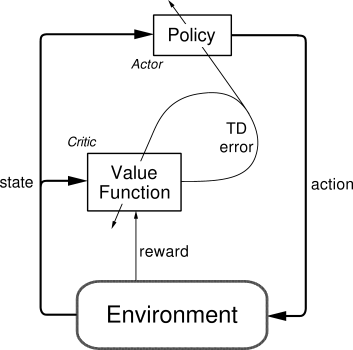
\includegraphics[width = 0.35\columnwidth]{figs/actorcritic.png}
 \caption{Actor Critic system. Reprinted from~\cite{sutton1998reinforcement}}
\label{fig:actorcriticsystem}
\end{figure}



